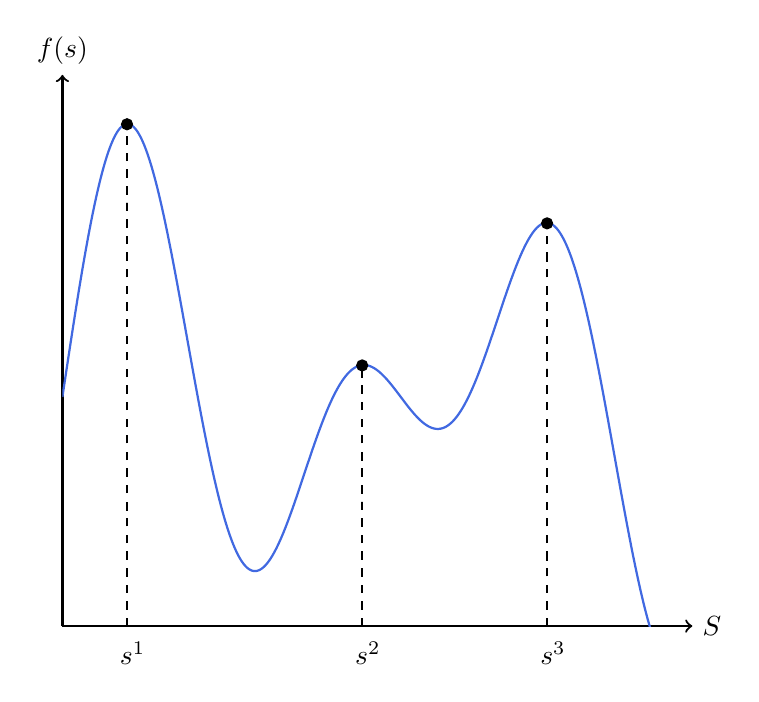
\begin{tikzpicture}
	% Axis Lines
	\draw[->, thick] (0,0) -- (8,0) node[right] {$S$};
	\draw[->, thick] (0,0) -- (0,7) node[above] {$f(s)$};

	\begin{axis}[axis lines = none,scale only axis=true,xmin=0,
			xmax=18.5,ymin=0,ymax=10]

		% Main Plot
		\addplot[domain=0:17,samples=1000,smooth,color=RoyalBlue,
			thick] {2.5*sin(deg(x)) + 2.5*sin(deg((2/3)*x)) + 4};

		% Vertical Line (s1)
		\addplot[domain=0:17,thick,samples=1000,dashed,
			smooth] coordinates {(1.8,0) (1.8,8.76)};
		\addplot[domain=0:17,mark=*] coordinates {(1.8,8.76)};
		% \draw (1.8,8.76) circle[radius=1.5pt];
		% \fill (1.8,8.76) circle[radius=1.5pt];

		% Vertical Line (s2)
		\addplot[domain=0:17,thick,samples=1000,dashed,
			smooth] coordinates {(8.35,0) (8.35,4.55)};
		% \draw (8.35,4.55) circle[radius=1.5pt];
		% \fill (8.35,4.55) circle[radius=1.5pt];
		\addplot[domain=0:17,mark=*] coordinates {(8.35,4.55)};

		% Vertical Line (s3)
		\addplot[domain=0:17,thick,samples=1000,dashed,
			smooth] coordinates {(13.5,0) (13.5,7.03)};
		% \draw (13.5,7.03) circle[radius=1.5pt];
		% \fill (13.5,7.03) circle[radius=1.5pt];
		\addplot[domain=0:17,mark=*] coordinates {(13.5,7.03)};
	\end{axis}

	% Labels
	\node (s1) at (0.89,-0.35) {$s^1$};
	\node (s1) at (3.88,-0.35) {$s^2$};
	\node (s1) at (6.23,-0.35) {$s^3$};

\end{tikzpicture}

